\section*{Results}

%\subsection*{Two-Choice Rule Switching Task}
Eighteen adult male mice were trained to high proficiency on a two-choice sensorimotor decision making task under head fixation (Fig. \ref{fig:Fig1}A--B). The task consisted of a set of trials in which subjects could choose between two stainless steel lick-ports placed on either side of the mouth, only one of which (the target) would provide a water reward when chosen. A sound cue presented at the start of each trial---either an upsweep or downsweep---indicated the target side (left for upsweeps, right for downsweeps).

\begin{figure}[htbp]

\begin{center}
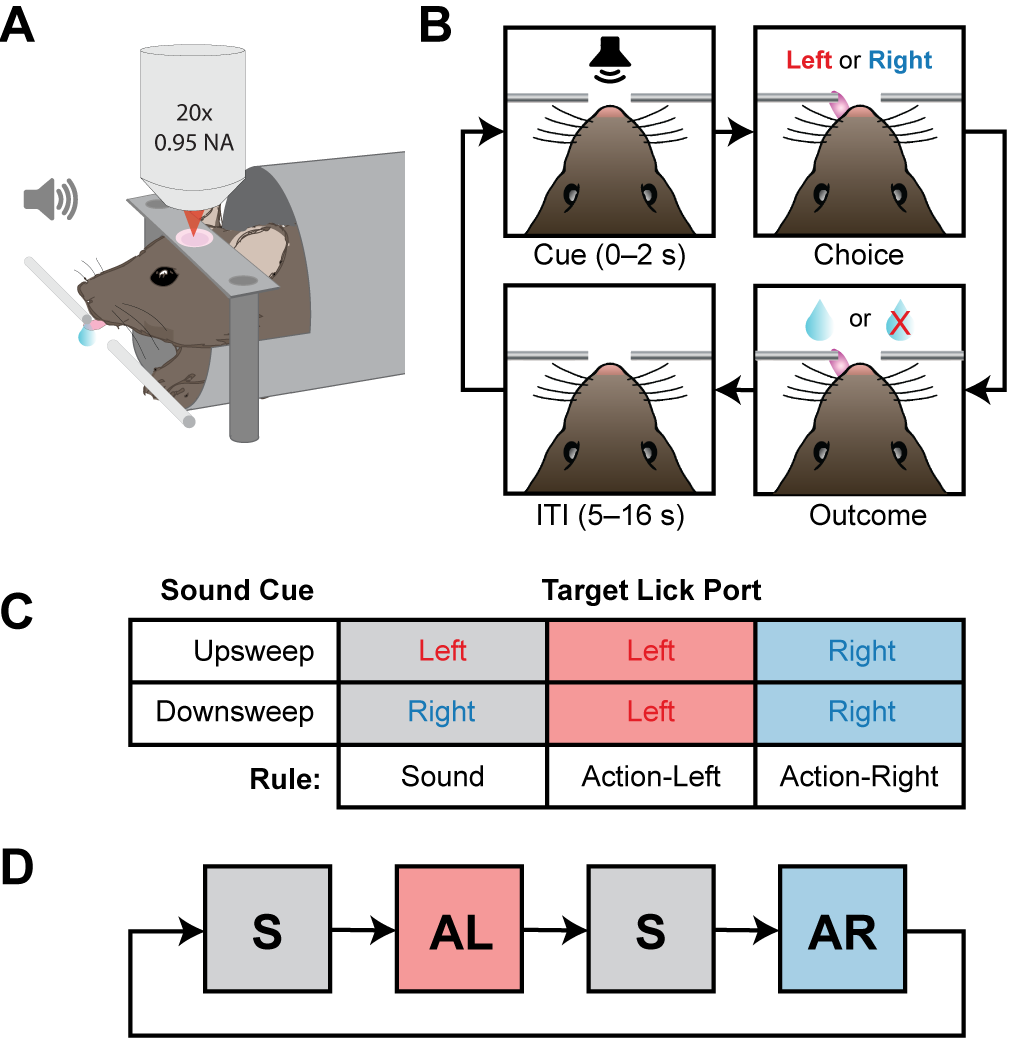
\includegraphics[width=8.7cm]{Figures/Fig1.png} 
\end{center}

\caption[Rule switching task for head-fixed mice.]
{Rule switching task for head fixed mice. (A) Experimental setup for two-choice sensorimotor task with simultaneous two-photon imaging. Mice rested inside of a stainless steel tube, with the head immobilized using a cranial implant. Two lick ports were placed on either side of the mouth to deliver water rewards. (B) Flow diagram of trial structure. A sound cue was played at the start of each trial, indicating the target port that would be rewarded (left or right). To obtain the reward, subjects were required to lick the target within 2 s following cue onset. After a random intertrial interval (ITI) of 5--16 s, a new sound cue was presented, providing a fresh opportunity to lick for a reward. (C) Table indicating the target lick port signified by each sound cue in each rule context. (D) Flow diagram of session structure. Trials governed by each rule were organized into blocks. Sound blocks (S) were interleaved with action blocks that alternated between the action-left (AL) and action-right (AR) rule. A new rule block was initiated on the next trial after an accuracy criterion was met (85\% for the past 20 trials of the current block).}

\label{fig:Fig1}
\end{figure}

Subjects were immediately rewarded with $\sim$ 2 \si{\uL} of water if the target port was chosen within 2 s of cue onset (a hit). Choosing the non-target port (an error) resulted in playback of a mild white noise sound. After a random interval of 5--16 seconds, the next cue was played, providing the opportunity to make another choice. New trials were generated until the subject failed to respond (missed) for twenty consecutive trials.

After meeting a performance criterion (three consecutive sessions at $>85\%$  accuracy), subjects were challenged with a modified version of this task, which was designed to elicit flexible sensorimotor decisions. Namely, the fixed relationship between each sound cue and its corresponding target was replaced with three alternative rules for action selection (Fig. \ref{fig:Fig1}C). 

In the sound rule, upsweeps signified a left target, and downsweeps signified a right target as described above. In the action-left rule, the target on every trial was the left port, regardless of whether upsweeps or downsweeps were presented. Conversely, under the action-right rule, the right port was always the target, irrespective of the auditory cue. 

Sessions were structured into alternating blocks of sound and action trials, such that each rule was enforced for at least 20 trials at a time (Fig. \ref{fig:Fig1}D). After 20 consecutive trials with $\geq 85\%$  accuracy, a rule-switch would occur---ie, a new rule block would begin on the next trial.

Subjects participated in $4 \pm 0$ sessions each (range: 2--5; $N=18$ mice), for a total of 65 sessions. Within each session, they completed an average $6 \pm 0$ rule blocks over the course of $561 \pm 21$ trials (all descriptive statistics are reported as $mean \pm SEM$; unless otherwise noted, the sample size $N$ is given by the number of sessions).

We used cellular resolution calcium imaging in layer 2/3 of M2 to separately measure the activity of SST, PV, VIP, and PYR neurons while subjects participated in the task. Imaging was restricted to the cell-type of interest in each experiment using one of three approaches. To target GABAergic interneurons (SST, PV, or VIP), we used transgenic mice that selectively express cyclic recombinase (cre) in the cell-type of interest \citep{taniguchi11}. In some cases ($N =$ 5 \emph{SST-cre} and 2 \emph{PV-cre} mice), an adeno-associated virus (AAV) encoding a cre-dependent GCaMP6s construct (AAV1-hSyn-Flex-GCaMP6s-WPRE-SV40) was injected into M2. In other cases, experimental subjects were F1 hybrids produced by crossing the cre-driver line with a second transgenic mouse line, \emph{Ai148} \citep{daigle18}, that expresses GCaMP6f in a cre-dependent manner ($N =$ 5 \emph{VIP-cre;Ai148} mice and 1 \emph{PV-cre;Ai148} mouse). To target pyramidal (PYR) neurons, we injected an AAV that encodes GCaMP6f under control of the CaMKII promoter (AAV1-CaMKII-GCaMP6f-WPRE-SV40; $N = 5$) \citep{kuchibhotla17, ali20}.

We visually identified a total of \num{5012} GCaMP\textsuperscript{+} neurons across all imaging sessions (Supplementary Table \ref{tab:expTable}). After excluding \num{1006} cells in which the baseline fluorescence was dimmer on average than that of the background (see Methods), we obtained cellular fluorescence time series from a total of 305 SST, 479 VIP, 263 PV, and 2959 PYR neurons. On average, $22 \pm 1$ SST, $25 \pm 1$ VIP, $22 \pm 2$ PV, or $148 \pm 9$ PYR neurons were included per session ($N =$ 14, 19, 12, and 20 sessions, respectively). The number of completed rule-blocks per session was similar during recordings from all cell-types, at $6 \pm 0$ for SST, VIP,  and PYR, and $7 \pm 1$ for PV ($F(3,61)=0.35$, $p=0.79$, 1-way ANOVA).      


\subsection*{Dependence of Lick Output on Task Structure}
As expected, the pattern of licking output was dependent on the task structure. Overall lick density varied based on elapsed time within the trial, as well as trial outcome (Fig. \ref{fig:Fig2}A--B). Specifically, the mean lick rate in completed trials increased from $0.8 \pm 0.1$ Hz in the 2 s prior to cue onset ("pre-cue"), to $2.6 \pm 0.1$ Hz in the 2 s following it ("post-cue"; paired $t(64) =38.9$, $p=\num{3e-46}$). The mean lick rate post-cue was higher for hits ($3.3 \pm 0.1$ Hz) than errors ($1.3 \pm 0.0$ Hz; paired $t(64) =24.6076$, $p=\num{2e-34}$),\ which likely reflects differences in consummatory licking.

\begin{SCfigure*}[][tbp]

% \begin{center}
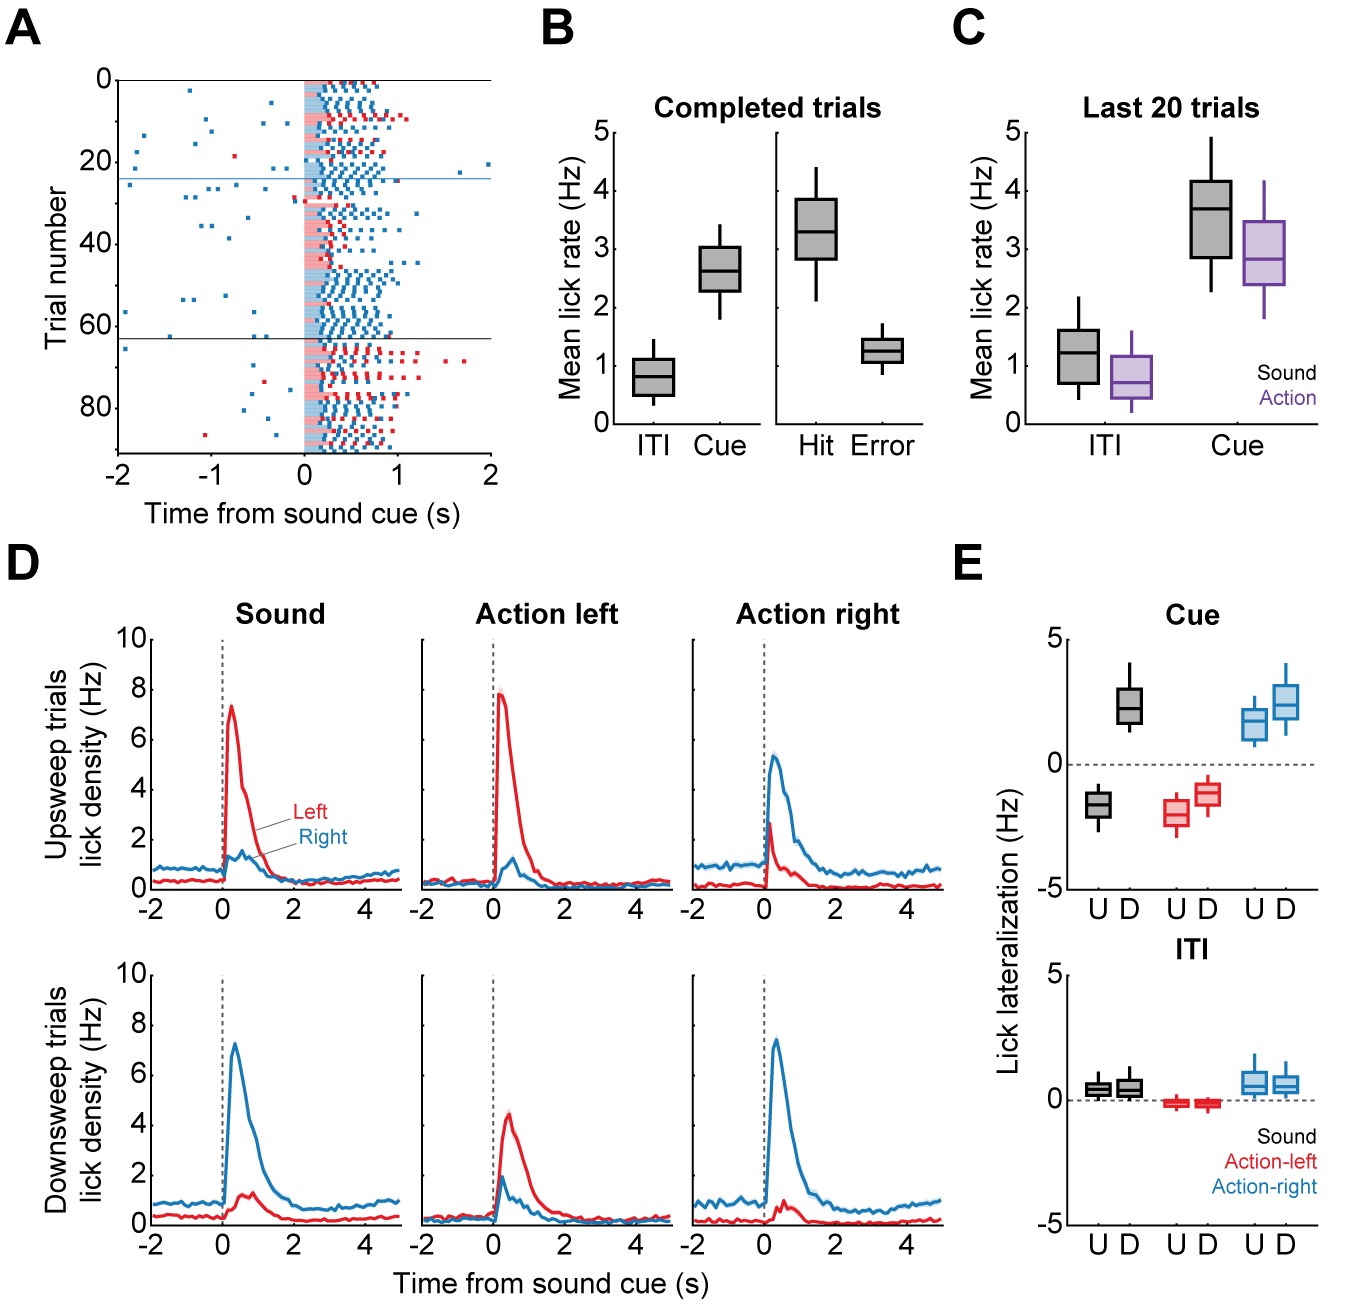
\includegraphics[width=11.4cm]{Figures/Fig2.png} 
% \end{center}

\caption[Dependence of lick output on task structure.]
{Dependence of lick output on the task structure. (A) Raster plot of individual lick times, aligned to cue onset during the first three blocks of an example session. Rows of the raster correspond to consecutive trials. The cue period of each trial is highlighted in pale red for upsweeps and pale blue for downsweeps, with red and blue tick marks representing left and right licks, respectively. Fine horizontal lines indicate the first trial of each rule block. The order of the blocks was sound--action-right--sound. (B) Mean lick rates for the 2 s periods before and after cue onset (ITI and Cue, respectively), estimated from all completed trials. Left, overall comparison of ITI and cue periods. Right, comparison of hit and error trials during the cue period. (C) Mean lick rates for the ITI and cue periods, presented separately for sound (black) and action trials (purple). (D) Mean lick density at the left (red) and right port (blue) across all sessions, calculated in 100 ms time bins surrounding cue onset. Data are plotted separately for upsweep (top) and downsweep trials (bottom) within each block type. Shading, SEM. (E) Lick lateralization in upsweep (U) and downsweep trials (D) within each block type. Lick lateralization was calculated as the difference between the number of right and left licks during the 2 s before (bottom) and after cue onset (top) in each trial. Positive and negative values indicate a greater number of right and left licks, respectively. For B--E, $N = 65$ sessions. For C--E, analysis was restricted to the last twenty trials of each block: the period in which the accuracy criterion was met. Box-and-whisker plots in all figures indicate the 9th, 25th, 50th, 75th, and 91st percentiles for each group.}

\label{fig:Fig2}
\end{SCfigure*}


An important difference between sound and action trials is that a conditional mode of action selection \citep{mitz91} is optimal under the sound rule; ie, only under the sound rule should choices depend on the identity of the sound cue. By contrast, the two action rules prescribe an unconditional mode of action selection that does not depend on cue identity. Therefore, in principle, correct choices could be made and even acted upon prior to cue onset in action trials, leading to rule-dependent differences in anticipatory licking.

To examine differences across rule types, we limited our analyses to the last twenty trials of each rule block---the period where at least 85$\%$  of choices were consistent with the corresponding rule. The mean pre-cue lick rate in action trials ($0.9 \pm 0.1$Hz) was no greater than in sound trials ($1.2 \pm 0.1$Hz; Fig. \ref{fig:Fig2}C). Moreover, the mean lick rate increased substantially upon cue onset in both sound and action trials (sound: $\Delta=2.4$Hz, paired $t(64) =29.0$, $p=\num{2e-38}$; action: $\Delta=2.0$ Hz, paired $t(64)=29.9$, $p=\num{3e-39}$). Thus, the overall pattern of licking output was largely conserved across rule types, despite fundamental differences in their temporal constraints on action selection (Fig. \ref{fig:Fig2}D).

Sound, action-left, and action-right rules are defined by the instructive content of each sound cue. Specifically, upsweeps and downsweeps signify diverging targets during sound blocks (left vs. right), and convergent but opposing targets during action-left and action-right blocks. Thus, choices should depend on an interaction between cue identity and the current rule. However, the choice made on a given trial concerns only the initial lick following the sound cue. To examine the extent to which the overall pattern of directional licking was structured by the task, we calculated a measure of lick lateralization by subtracting the mean left-lick rate from the mean right-lick rate during the post-cue period of each trial. For example, in sound trials, relative lick density was $-1.6 \pm 0.1$Hz following an upsweep, and $2.5 \pm 0.1$Hz following a downsweep.

We examined the dependence of this measure on cue identity, block-type, and their interaction with a 2-way repeated measures ANOVA  (Fig. \ref{fig:Fig2}E). Individual comparisons were made using Tukey’s post hoc test. As expected, this analysis revealed a significant dependence of lick lateralization on the interaction between block type and cue identity ($F(2,128)=410$, $p=\num{4e-56}$). Specifically, lick lateralization following upsweeps versus downsweeps differed most during sound blocks ($\Delta=4.1$Hz, $p=\num{1e-10}$). A much smaller difference was observed during action blocks (action-left: $\Delta=0.8$Hz, $p=\num{1.1e-10}$; action-right: $\Delta=0.8$Hz, $p=\num{1.1e-10}$). 

An\ identical analysis considering the pre-cue period revealed a small but significant  rule-dependent difference in lick lateralization (sound: $0.5 \pm 0.1$ Hz, action-left: $-0.1 \pm 0.0$ Hz, action-right: $0.7 \pm 0.1$ Hz; $F(2,128) =100$, $p=4e-27$). As expected, neither the cue identity ($F(1,64) =0.39$, $p=0.54$) nor the interaction of cue identity and block type ($F(2,128) =1.6$, $p=\num{0.22}$) were significant predictors of relative lick density during the pre-cue period.

\subsection*{Formal Measures of Task Performance}
Excluding the initial sound block, an average of $88 \pm 3$ trials were required to reach the accuracy criterion that triggered a rule switch (20 consecutive trials at $ \geq 85\%$ accuracy). Mean accuracy was slightly above criterion, at $86 \pm 0 \%$ during the final twenty trials of a rule block. Perseverative errors, defined as choices consistent with the previous rule but inconsistent with the current rule, were substantially more frequent than other errors. Specifically, $26 \pm 1$ perseverative errors and $3 \pm 0$ other errors were committed per block. The difference was significant in both sound ($\Delta=6$, paired $t(64) =8.2$, $p=\num{2e-11}$) and action blocks ($\Delta=38$, paired $t(64) =18.7$, $p=\num{1e-27}$).

\begin{figure}[htbp]

\begin{center}
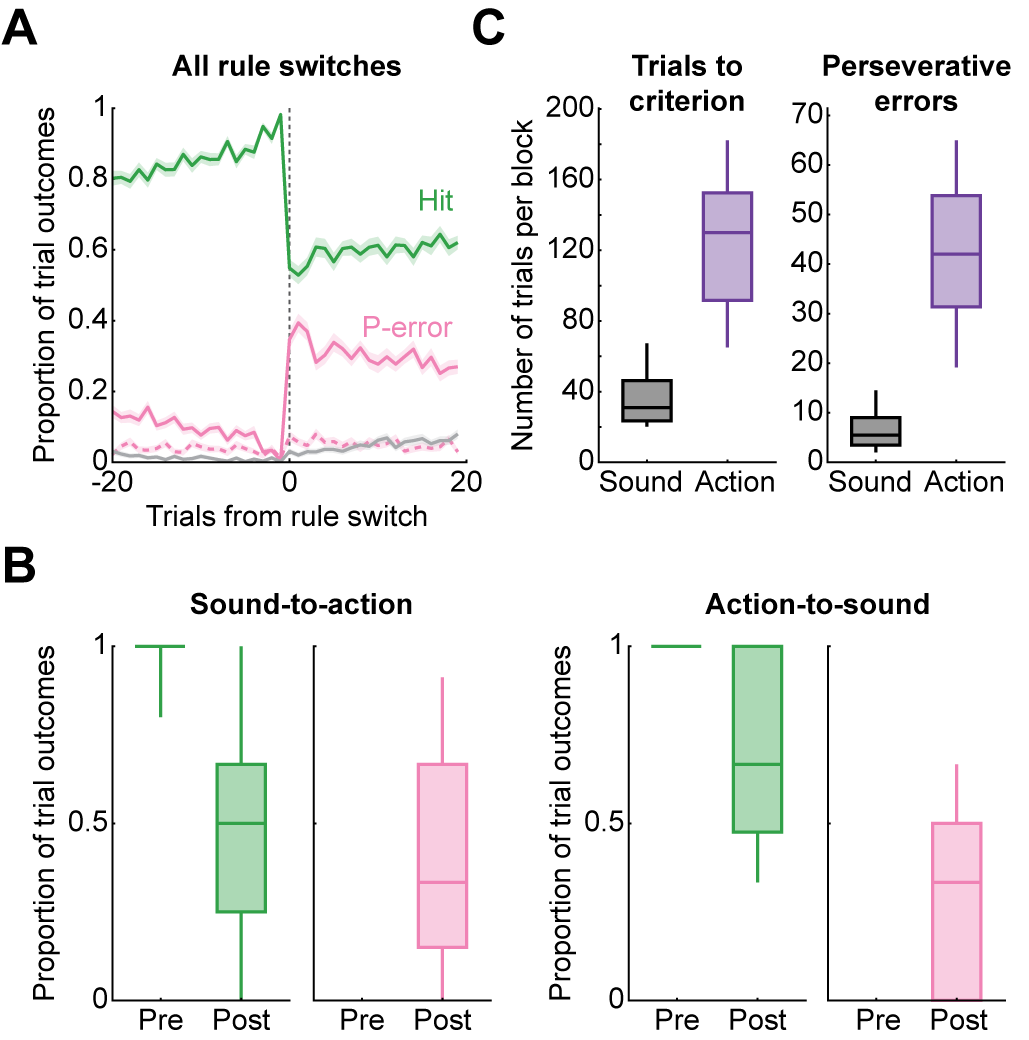
\includegraphics[width=8.7cm]{Figures/Fig3.png} 
\end{center}

\caption[Formal measures of task performance.]
{Formal measures of task performance. (A) Mean proportion of hits (green), perseverative errors (solid pink), other errors (dashed pink), and misses (gray) as a function of the number of trials from a rule switch across all sessions ($N=65$). Shading, SEM. (B) Boxplots representing the mean proportion of hits (green) and preseverative errors (pink) for trials immediately preceding a rule switch (Pre) and for trials immediately following one (Post). Results are presented separately for switches from the sound rule to an action rule (left), and vice-versa (right). (C) Boxplots representing the number of trials taken to reach criterion (left), and the number of perseverative errors committed (right), during sound (black) and action blocks (purple). All boxes indicate quartiles 1--3; whiskers indicate 9th and 91st percentiles.}

\label{fig:Fig3}
\end{figure}

As expected, accuracy dropped precipitously following a rule switch (\ref{fig:Fig3}A). The proportion of hits decreased from $98 \pm 1 \%$ in the trial before a rule switch, to $55 \pm 2 \%$ in the next trial (paired $t(64) =16.9$, $p=\num{3e-25}$). This reduction in accuracy was mostly attributable to an increase in perseverative errors, which accounted for $0 \pm 0 \%$ of trials immediately preceding a rule switch and $35 \pm 2 \%$ of trials immediately following (paired $t(64) =13.7$, $p=\num{9e-21}$). A much smaller increase was noted in the proportion of other errors ($\Delta=6\%$, paired $t(64) =3.8$, $p=\num{3e-4}$) and misses ($\Delta=3\%$, paired $t(64) =3.7$, $p=\num{5e-4}$). 

Results of this analysis are presented separately for switches from the sound rule to an action rule, and vice-versa, in Figure \ref{fig:Fig3}B. In both cases, the proportion of hits decreased substantially in the trial following a rule switch (sound-to-action: $\Delta=51\%$, paired $t(64) =12.6$, $p=\num{5e-19}$; action-to-sound: $\Delta=34\%$, paired $t(64) =8.7$, $p=\num{2e-12}$). Following a sound-to-action rule switch, the proportion of hits was indistinguishable from chance, at $46 \pm 4 \%$ ($t(64)=1.0$, $p=0.30$; one-sample t-test for the null hypothesis, $H_0:\Delta=0.5$), but remained significantly above chance following an action-to-sound rule switch ($mean=66 \pm 4 \%$, one-sample $t(64)=4.1$, $p=\num{1e-4}$). In both cases, the proportion of perseverative errors increased significantly (sound-to-action: $\Delta=39\%$, paired $t(64) =9.9$, $p=\num{1e-14}$; action-to-sound: $\Delta=29\%$, paired $t(64) =8.5$, $p=\num{4e-12}$).  

Although subjects were capable of adjusting their sensorimotor decisions to both rule types, in general, they adapted more readily during action-to-sound rule transitions than the reverse (Fig. \ref{fig:Fig3}C). During sound blocks, substantially fewer trials were taken to reach the accuracy criterion ($39 \pm 3$ vs. $126 \pm 6$; paired $t(64) =13.4$, $p=\num{3e-20}$), and fewer perseverative errors were committed before the criterion was reached ($7 \pm 1$ vs. $43 \pm 2$; paired $t(64) =14.3$, $p=\num{1e-21}$).

\subsection*{Task-Related Modulation of Neural Activity}


\subsubsection*{Choice-Related Modulation}

\subsubsection*{Outcome-Related Modulation}

\subsubsection*{Context-Related Modulation}